\documentclass[10pt]{article}

\usepackage[margin=1in]{geometry}
\usepackage{amsmath}
\usepackage{amssymb}
\usepackage{amsthm}
\usepackage{mathtools}
\usepackage{bm}
\usepackage{tikz}

\usepackage{color}
\usepackage{colortbl}
\definecolor{deepblue}{rgb}{0,0,0.5}
\definecolor{deepred}{rgb}{0.6,0,0}
\definecolor{deepgreen}{rgb}{0,0.5,0}
\definecolor{gray}{rgb}{0.7,0.7,0.7}
\definecolor{lightgray}{rgb}{0.7,0.7,0.7}

\usepackage{booktabs}
\usepackage{array}
\newcolumntype{L}[1]{>{\raggedright\let\newline\\\arraybackslash\hspace{0pt}}m{#1}}
%\newcolumntype{C}[1]{>{\centering\let\newline\\\arraybackslash\hspace{0pt}}m{#1}}
%\newcolumntype{C}[1]{>{\centering\arraybackslash}m{#1}}
\newcolumntype{C}[1]{>{\centering\arraybackslash}m{#1}}
\newcolumntype{R}[1]{>{\raggedleft\let\newline\\\arraybackslash\hspace{0pt}}m{#1}}
%\newcolumntype{A}[2]{%
    %>{\minipage{\dimexpr#1\linewidth-2\tabcolsep-#2\arrayrulewidth\relax}\vspace\tabcolsep}%
    %c<{\vspace\tabcolsep\endminipage}}

\usepackage{hyperref}
\hypersetup{
  colorlinks   = true, %Colours links instead of ugly boxes
  urlcolor     = black, %Colour for external hyperlinks
  linkcolor    = blue, %Colour of internal links
  citecolor    = blue  %Colour of citations
}

%%%%%%%%%%%%%%%%%%%%%%%%%%%%%%%%%%%%%%%%%%%%%%%%%%%%%%%%%%%%%%%%%%%%%%%%%%%%%%%%

\theoremstyle{definition}
\newtheorem{problem}{Problem}
\newtheorem{defn}{Definition}
\newcommand{\R}{\mathbb R}
\DeclareMathOperator{\vcdim}{VCdim}
\DeclareMathOperator{\E}{\mathbb E}
\DeclareMathOperator{\nnz}{nnz}
\DeclareMathOperator{\determinant}{det}
\DeclareMathOperator{\Var}{Var}
\DeclareMathOperator{\rank}{rank}
\DeclareMathOperator*{\argmin}{arg\,min}
\DeclareMathOperator*{\argmax}{arg\,max}

\newcommand{\I}{\mathbf I}
\newcommand{\Q}{\mathbf Q}
\newcommand{\p}{\mathbf P}
\newcommand{\pb}{\bar {\p}}
\newcommand{\pbb}{\bar {\pb}}
\newcommand{\pr}{\bm \pi}
\newcommand{\epsapp}{\epsilon_{\text{app}}}
\newcommand{\epsest}{\epsilon_{\text{est}}}

\newcommand{\trans}[1]{{#1}^{T}}
\newcommand{\loss}{\ell}
\newcommand{\w}{\mathbf w}
\newcommand{\x}{\mathbf x}
\newcommand{\y}{\mathbf y}
\newcommand{\lone}[1]{{\lVert {#1} \rVert}_1}
\newcommand{\ltwo}[1]{{\lVert {#1} \rVert}_2}
\newcommand{\lp}[1]{{\lVert {#1} \rVert}_p}
\newcommand{\linf}[1]{{\lVert {#1} \rVert}_\infty}
\newcommand{\lF}[1]{{\lVert {#1} \rVert}_F}

\newcommand{\h}{\mathcal H}
\newcommand{\D}{\mathcal D}
\DeclareMathOperator*{\erm}{ERM}
\DeclareMathOperator*{\sign}{sign}

\newcommand{\ignore}[1]{}

%%%%%%%%%%%%%%%%%%%%%%%%%%%%%%%%%%%%%%%%%%%%%%%%%%%%%%%%%%%%%%%%%%%%%%%%%%%%%%%%

\begin{document}


\begin{center}
\Huge
Notes: Stochastic Gradient Descent II
\end{center}

\begin{center}
    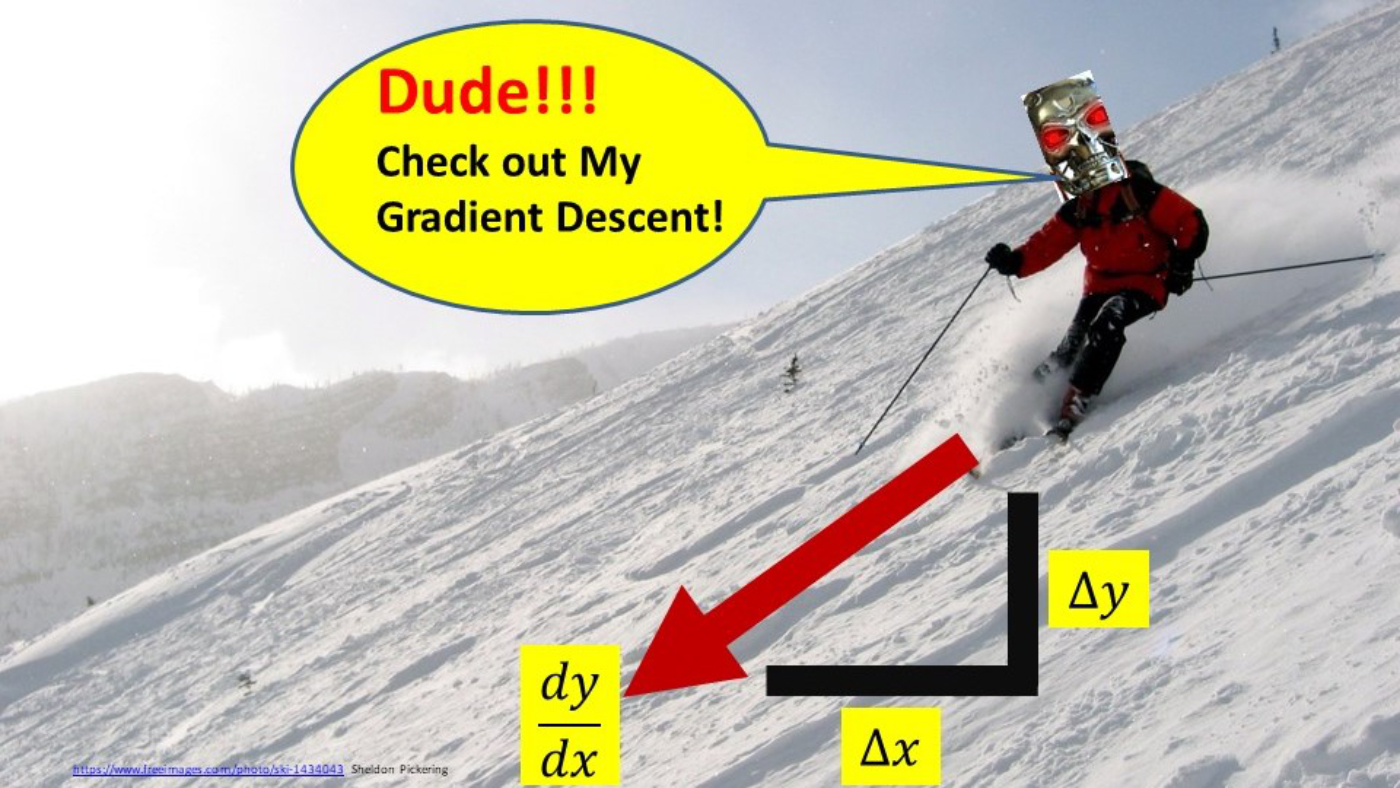
\includegraphics[height=3in]{skiing.jpg}
\end{center}

%%%%%%%%%%%%%%%%%%%%%%%%%%%%%%%%%%%%%%%%%%%%%%%%%%%%%%%%%%%%%%%%%%%%%%%%%%%%%%%%

\section{Pre-lecture Work}

\begin{problem}
    I recommend watching the following StatQuest videos if you are unfamiliar with either gradient descent or stochastic gradient descent.
    \begin{enumerate}
        \item Gradient descent: \url{https://www.youtube.com/watch?v=sDv4f4s2SB8}
        \item Stochastic gradient descent: \url{https://www.youtube.com/watch?v=vMh0zPT0tLI}
    \end{enumerate}
    The following StatQuest videos about regularization may also be helpful:
    \begin{enumerate}
        \item L2 regularization: \url{https://www.youtube.com/watch?v=Q81RR3yKn30}
        \item L1 regularization: \url{https://www.youtube.com/watch?v=NGf0voTMlcs}
        \item Elastic-net regularization: \url{https://www.youtube.com/watch?v=1dKRdX9bfIo}
    \end{enumerate}
\end{problem}

\begin{problem}
    Before the \emph{2nd day of lecture},
    you should complete all the problems marked with a $\star$.
\end{problem}

%%%%%%%%%%%%%%%%%%%%%%%%%%%%%%%%%%%%%%%%%%%%%%%%%%%%%%%%%%%%%%%%%%%%%%%%%%%%%%%%
\newpage
\section{Lecture Warm-up}

\begin{problem}
    Recall that in a regression problem,
    feature vectors are contained in the space $\mathcal X=\R^d$,
    and the prediction space is $\mathcal Y = \R$.
    In Tikhonov regression,
    we use the squared loss and the L2 regularizer.
    The resulting minimization problem is
    \begin{equation}
        \hat \w = \argmin_\w \tfrac 1 m \sum_{i=1}^m \tfrac 1 2 (\trans\w \x_i - y)^2 + \lambda \ltwo{\w}^2.
    \end{equation}
    \begin{enumerate}
        \item Find a closed form solution for $\hat \w$.
            \vspace{4in}
        \item What is the runtime of computing the above expression?
            \vspace{1in}
        \item Why is there a closed form solution for $\hat \w$?
    \end{enumerate}
\end{problem}

%%%%%%%%%%%%%%%%%%%%%%%%%%%%%%%%%%%%%%%%%%%%%%%%%%%%%%%%%%%%%%%%%%%%%%%%%%%%%%%%
\newpage
\section{Lecture}
\begin{problem}
    Convex-Lipschitz Gradient Descent.
    \begin{enumerate}
        \item The update rule (Eq. 14.1)
            \newpage
        \item Corollary 14.2 (convergence rate)
            \vspace{4in}
        \item How should we choose $\epsilon$ and $T$?
    \end{enumerate}
\end{problem}

\newpage
\begin{problem}
    Lipschitz Stochastic Gradient Descent.
    \begin{enumerate}
        \item The update rule (Section 14.3)
            \newpage
        \item ($\star$) Definition 12.12 (convex-lipschitz-bounded learning problem)
            \vspace{4.5in}
        \item ($\star$) Theorem 14.8  (optimization convergence rate)
            \vspace{4.5in}
        \item ($\star$) Corollary 14.12 (learning convergence rate)
    \end{enumerate}
\end{problem}

\newpage
\begin{problem}
    Convex Smooth Stochastic Gradient Descent.
    \begin{enumerate}
        \item 
            The update rule is the same as in the Lipschitz case.
            The only difference is the analysis.
        \item ($\star$) Definition 12.13 (convex-smooth-bounded learning problem)
            \vspace{4in}
        %\item ($\star$) Theorem 14.11 (optimization convergence rate)
            %\vspace{4in}
        \item ($\star$) Corollary 14.14 (learning convergence rate)
    \end{enumerate}
\end{problem}

\newpage
\begin{problem}
    Strongly Convex Stochastic Gradient Descent.
    \begin{enumerate}
        \item 
            The update rule is the same as in the Lipschitz case.
            The only difference is the analysis.
            In this case, the book presents the analysis in just a single theorem.
        \item ($\star$) Theorem 14.11 (optimization convergence rate)
    \end{enumerate}
\end{problem}

%%%%%%%%%%%%%%%%%%%%%%%%%%%%%%%%%%%%%%%%%%%%%%%%%%%%%%%%%%%%%%%%%%%%%%%%%%%%%%%%
\newpage
\section{Learning Problems}
\begin{problem}
    Consider the classification problem using the logistic loss with no regularization.
    \begin{enumerate}
        \item 
            What are the SGD generalization bounds?
            \newpage
        \item 
            Now assume that L2 regularization is used.
            What are the new generalization bounds for SGD?
            \newpage
        \item 
            Now assume that L1 regularization is used.
            What is the new generalization bounds for SGD?
    \end{enumerate}
\end{problem}

\newpage
\begin{problem}
    Consider the regression problem using the squared loss with no regularization.
    \begin{enumerate}
        \item 
            What are the SGD generalization bounds?
            \newpage
        \item 
            Now assume that L2 regularization is used.
            What are the new generalization bounds for SGD?
            \newpage
        \item 
            Now assume that L1 regularization is used.
            What is the new generalization bounds for SGD?
    \end{enumerate}
\end{problem}

\newpage
\begin{problem}
    (optional) 
    Repeat the above exercises using the absolute loss and Huber loss for regression problems, and the hinge loss and exponential loss for classification problems.
    Also consider elastic net regularization for all combinations of losses.
\end{problem}

\newpage
\begin{problem}
    This problem concerns generalization bounds for nearest neighbor algorithms.
    \begin{enumerate}
        \item ($\star$) Reproduce Theorem 19.3 (generalization bound of nearest neighbor)
        \vspace{4.5in}
        \item How does this result relate to the VC-dimension of nearest neighbor being infinite?
    \end{enumerate}
\end{problem}

\end{document}


